\section{Method}
\label{sec:method}
AtomVLA separates atomic execution into discrete intent, terminal geometry, and imagined evolution. A text head generates the atomic name and string-valued arguments; action Query supplies only the terminal end-effector pose. A future-imagination expert models the intermediate visual evolution that would otherwise be specified by a primitive's procedural body, and an action expert generates executable control. Figure~\ref{fig:overview} shows their shared MoT interface.

\begin{figure*}[t]
\centering
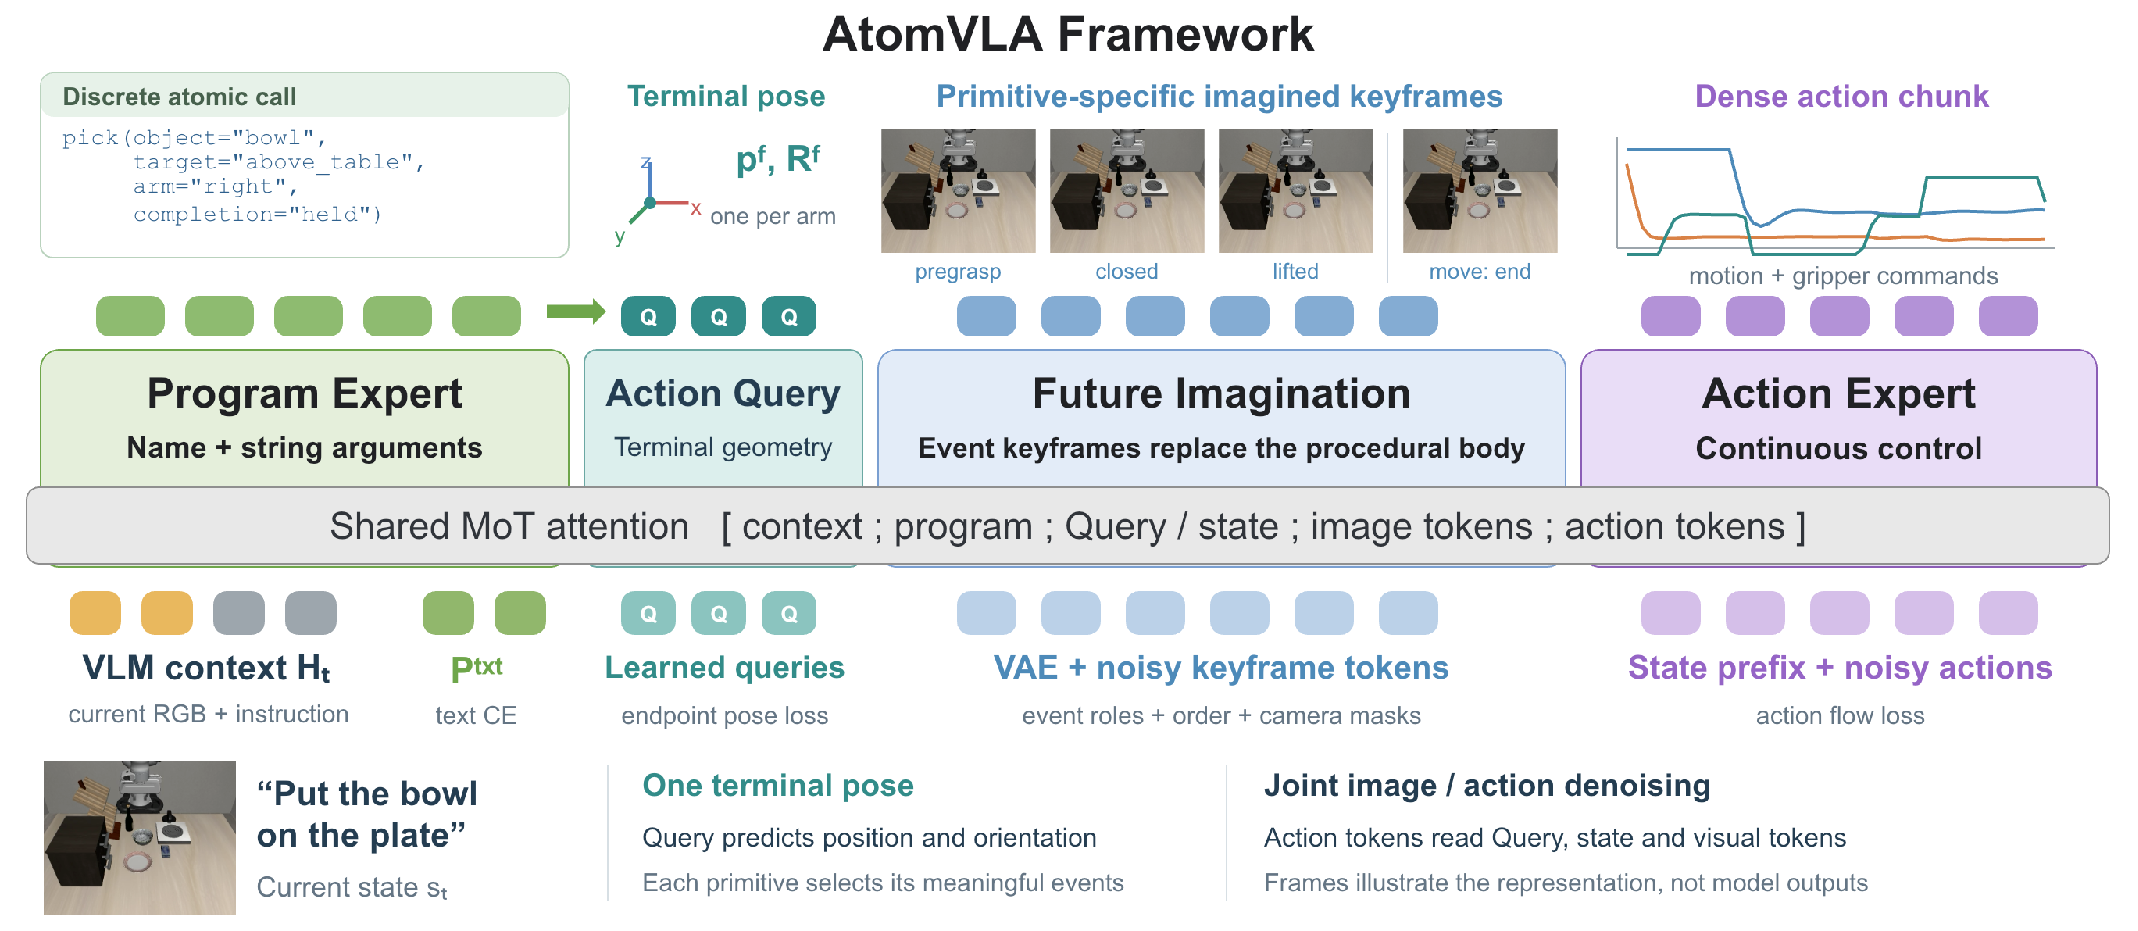
\includegraphics[width=\textwidth]{atomvla_framework.pdf}
\caption{\textbf{AtomVLA architecture.} The program expert emits an atomic name and string arguments. Action Query predicts only the terminal position and orientation per active arm. Future imagination represents within-primitive evolution as ordered visual states, replacing a generated executable function body. Concatenated image/action streams jointly denoise through MoT attention; action tokens read Query, robot state, and evolving visual tokens. Pick illustrates pregrasp, closure, and lift; move illustrates arrival. These are demonstration examples of different event structures, not measured predictions.}
\label{fig:overview}
\end{figure*}

\subsection{Dataset Annotation Pipeline}
\label{sec:data}
We align each demonstrated primitive with a discrete call, one terminal pose per active arm, an ordered future-image sequence, and action chunks. The call names an operation and uses strings for object, target, arm, contact mode, and completion condition. Only position and orientation are continuous call parameters; they are supervised separately through action Query. No executable function body is a prediction target. The semantic vocabulary follows the 16 Physical Words labels~\cite{physicalwords}; schemas and coverage conventions appear in Appendix~\ref{app:vocabulary}.

\begin{figure*}[t]
\centering
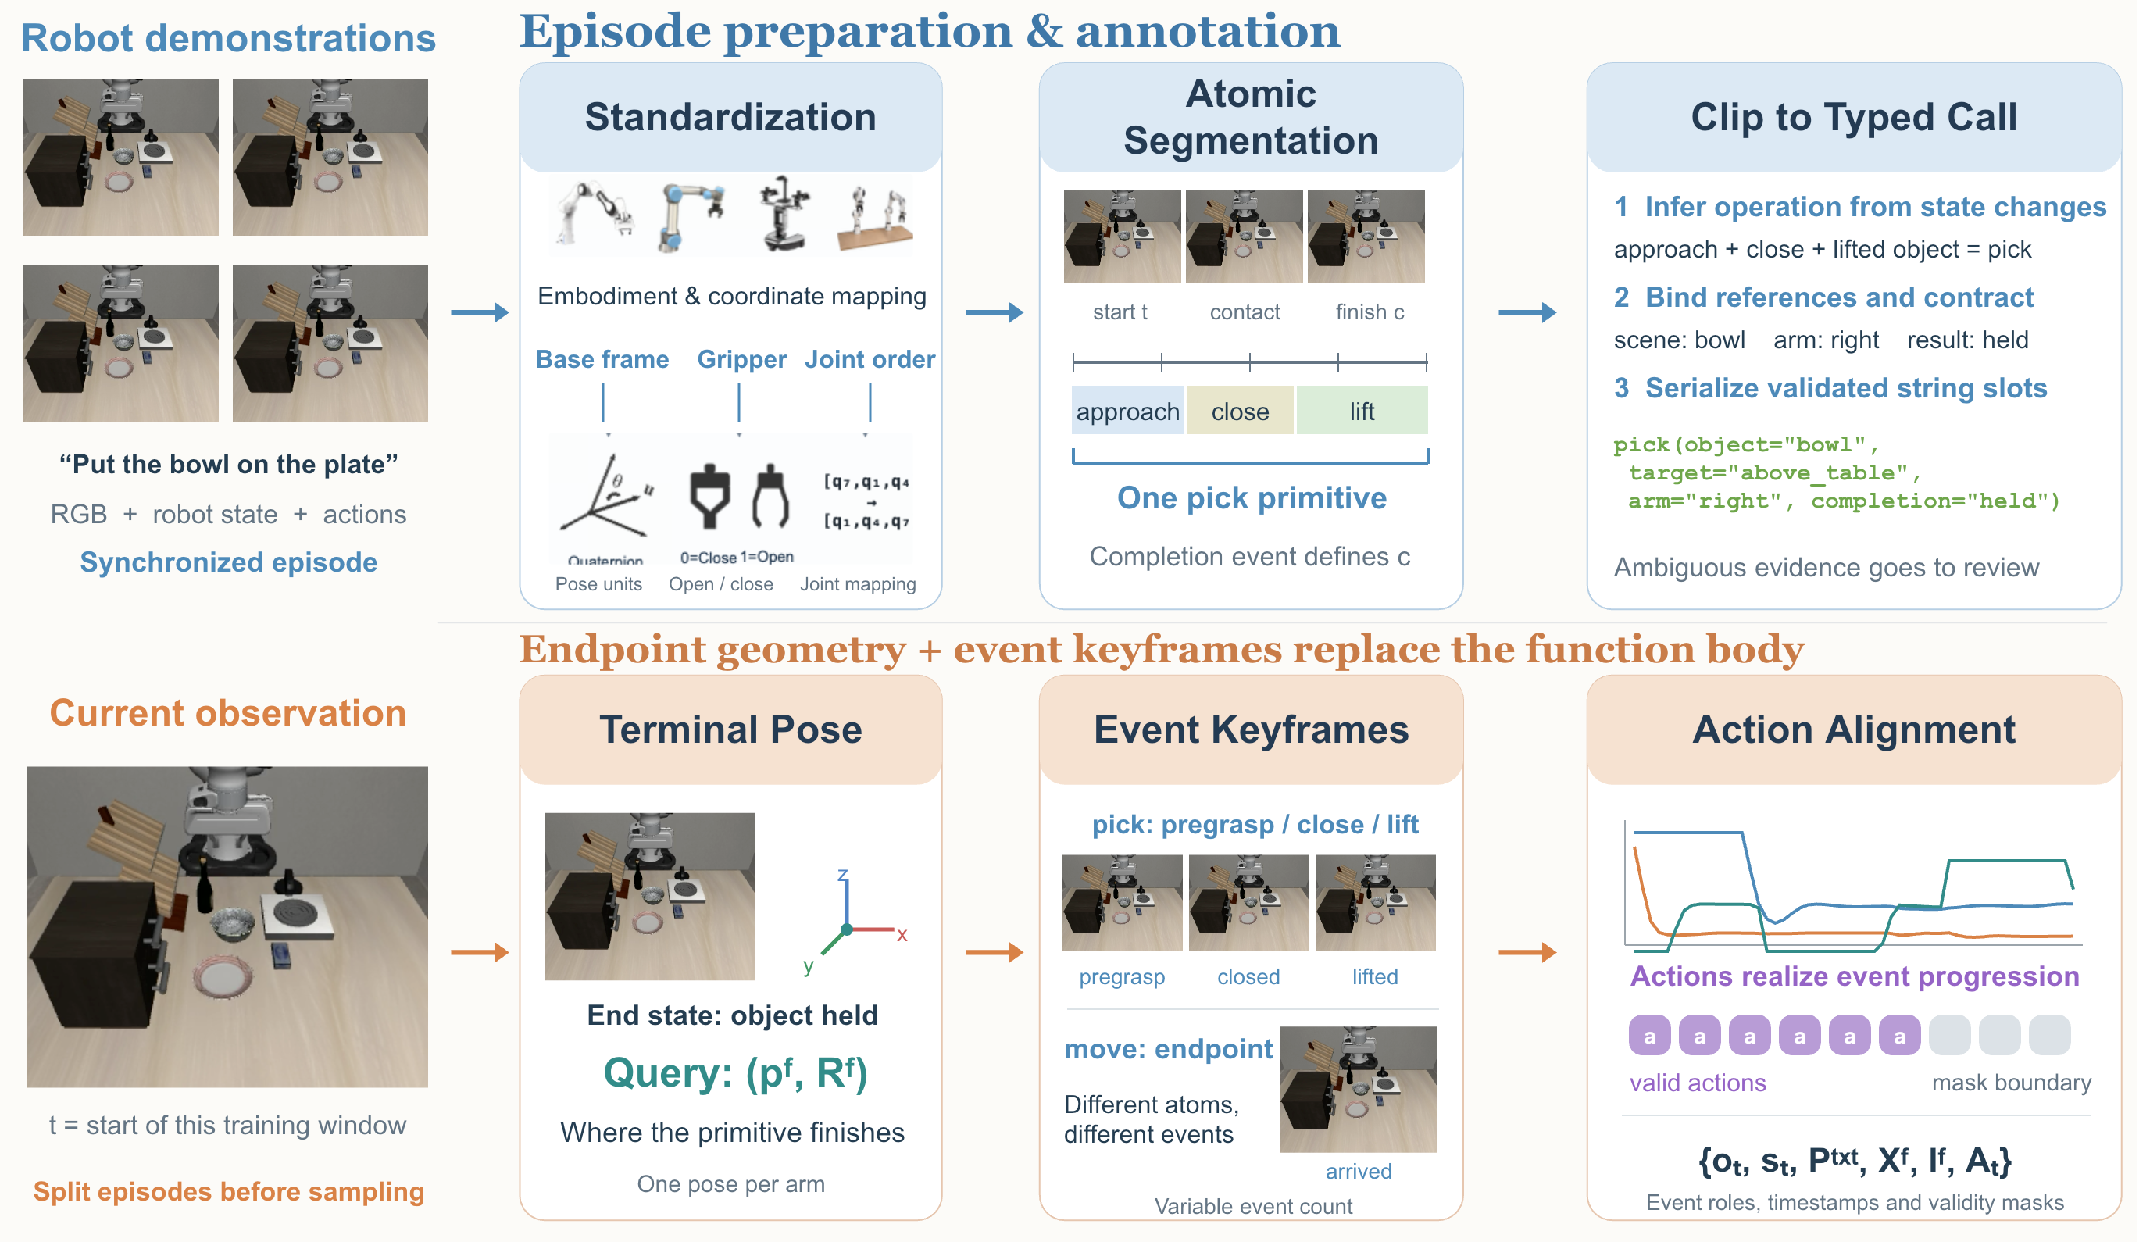
\includegraphics[width=\textwidth]{atomvla_annotation_pipeline.pdf}
\caption{\textbf{Dataset annotation pipeline.} The upper row standardizes synchronized demonstrations, identifies primitive intervals, then infers verbs from observed state changes, binds scene references, checks contracts, and serializes typed calls. The lower row aligns the current observation with a terminal pose, primitive-specific event frames, and demonstrated actions. Endpoint geometry and imagined events jointly replace the procedural body. The LIBERO images illustrate one pick interval within a bowl-placement episode; these are source demonstration frames, not model predictions.}
\label{fig:annotation}
\end{figure*}

\textbf{Clip-to-program conversion.} After synchronization and segmentation, we infer each operation from its observed state changes, ground object/target references in the scene, assign the arm, and check the completion contract. Approach, closure, and an object moving with the gripper support a single \texttt{pick} call. We serialize validated names and string slots; continuous terminal geometry remains a separate target. Ambiguous bindings, unverified events, and failed attempts enter review rather than acquiring successful labels.

\textbf{Multimodal target alignment.} For current time $t$ and verified completion $c(t)$, $X_t^F$ contains the terminal end-effector position and orientation. The call and observed phase determine meaningful event roles: \texttt{pick} uses pregrasp, closure, and lift, whereas a simple \texttt{move} can use arrival alone. Verified events give $t<\tau_1<\cdots<\tau_{K_i}=c(t)$ and $\mathcal I_t^F=(o_{\tau_1},\ldots,o_{\tau_{K_i}})$, with variable $K_i$ rather than uniform temporal sampling. A record is
\begin{equation}
\mathcal D_i=(o_t,l,s_t,P_t^{\rm txt},X_t^F,\mathcal I_t^F,A_t,\mu_i).
\label{eq:record}
\end{equation}
Metadata records timestamps, frames, arm/camera masks, and annotation quality. Both arms and all available cameras share the same temporal indices. Action chunks are truncated or masked at boundaries; invalid or failed outcomes receive no invented successful targets. Appendix~\ref{app:annotation} details temporal sampling and quality checks.

\subsection{Model and Training}
\label{sec:program}
\textbf{Discrete call and terminal Query.} The VLM encodes current inputs as $H_t$. Its text head predicts $P_t^{\rm txt}=(v_t,r_t,d_t,\kappa_t)$: the operation name, object/target references, other string arguments, and a string-valued completion condition. It generates neither numeric pose tokens nor function bodies. Learned Query tokens ground the terminal geometry:
\begin{equation}
Q_t=\operatorname{Query}(H_t,E_P(P_t^{\rm txt}),s_t),\quad
\widehat X_t^F=D_{\rm pose}(Q_t).
\label{eq:query}
\end{equation}
\label{sec:query}
The call's continuous parameters are the predicted terminal position and orientation in a calibrated robot-base frame, one pose per valid arm. Query does not predict intermediate waypoints, RGB, or motor commands. Its latent tokens and decoded terminal pose condition the downstream experts. Position and geodesic rotation losses supervise this endpoint without assuming that endpoint accuracy determines the path.

\textbf{Future imagination in MoT.}
\label{sec:mot}
The image expert predicts $\widehat{\mathcal I}_t^F$ from current context, the call, and terminal geometry. Pose specifies where the primitive finishes; imagined keyframes express its internal event progression. For \texttt{pick}, they describe pregrasp, closure, and lift. A simple \texttt{move} may require only arrival; contact or obstacle negotiation can require additional reviewed event schemas. Thus internal logic becomes a learned visual representation whose content and length depend on the primitive. The action expert realizes the dense motion between these states.

Image and action experts retain the concatenated MoT structure:
\begin{equation}
\begin{aligned}
C_t&=[H_t;E_P(P_t^{\rm txt});E_s(s_t);Q_t;E_X(\widehat X_t^F)],\\
Z_\sigma&=[C_t;E_I(\mathcal I_{t,\sigma}^F);E_A(A_{t,\sigma})].
\end{aligned}
\label{eq:motconcat}
\end{equation}
Event-role, order, and camera embeddings distinguish keyframes; padding carries no loss. At runtime, remaining roles follow the call schema and phase inferred from observations, never future annotations. The action stream attends to the evolving image tokens, together with Query and current state, to generate dense action chunks including gripper commands. Image/action tokens jointly denoise through modality-specific experts; the diagram's semantic dependence does not require a separate image-only rollout before every action. Clean future frames are never inference inputs, and current-context tokens cannot read future-target tokens. Appendix~\ref{app:losses} specifies the generation mask and losses.

\textbf{Training.} Warm-up trains the text head and Query/pose modules on aligned records with pretrained backbones frozen. Text cross-entropy supervises only the discrete call; all continuous call parameters are learned through terminal-pose supervision. Joint training then updates these modules, the image/action experts, and selected backbone adapters. Sequence RGB supervision teaches the imagined intermediate evolution, while demonstrated actions supervise physical control:
\begin{equation}
\mathcal L=\mathcal L_{\rm txt}+\lambda_p\mathcal L_{\rm pose}
+\lambda_i\mathcal L_{\rm seq}+\lambda_a\mathcal L_{\rm act}.
\label{eq:training}
\end{equation}
Losses use valid-target masks. Image and action losses also update the shared representation; the pose head receives no intermediate-waypoint regression objective. Joint batches mix annotated and decoded discrete calls, but downstream geometric conditioning always uses predicted Query outputs. Details and fixed-before-evaluation defaults appear in Appendix~\ref{app:training}.

\textbf{Closed-loop execution.} The model generates a discrete call, predicts its terminal pose, and imagines the within-primitive visual evolution while synthesizing actions. It executes a short action prefix, obtains new observations, and regenerates the remaining predictions. Observed completion advances to the next call; unmet conditions permit continued execution or re-grounding. Imagination is a learned forecast, not a correctness guarantee or a simulator. The action expert realizes motion and contact; robot-specific controllers execute its actions. Optional memory and feedback remain separately evaluated extensions.
